
%(BEGIN_QUESTION)
% Copyright 2011, Tony R. Kuphaldt, released under the Creative Commons Attribution License (v 1.0)
% This means you may do almost anything with this work of mine, so long as you give me proper credit

The {\it hydrocracking} process in oil refineries is exothermic, generating a lot of heat.  Temperature in the reactors is controlled by introducing hydrogen gas, which ``quenches'' the reaction by acting as a coolant.  In this reactor, three identical temperature transmitters are used to measure the same point inside the reactor, their signals selected by a median-select function (TY-24) before being passed on to the temperature controller.  Suppose the control system is functioning as it is designed to, under regular operating conditions as shown in this simplified diagram:

$$\includegraphics[width=15.5cm]{i01740x01.eps}$$

\noindent
Choose the best answer describing the immediate effect on this process if temperature transmitter TT-24a suddenly fails with a {\it low} (very cold) signal:

\begin{itemize}
\item{} The quench hydrogen valve (TV-24) will close slightly, attempting to raise temperature
\vskip 10pt
\item{} The quench hydrogen valve (TV-24) will open dramatically, attempting to lower temperature
\vskip 10pt
\item{} Nothing will happen.  The quench hydrogen valve (TV-24) will hold the exact same position
\vskip 10pt
\item{} The quench hydrogen valve (TV-24) will open slightly, attempting to lower temperature 
\end{itemize}

\underbar{file i01740}
%(END_QUESTION)





%(BEGIN_ANSWER)

The quench hydrogen valve (TV-24) will close slightly, attempting to raise temperature

%(END_ANSWER)





%(BEGIN_NOTES)

{\bf This question is intended for exams only and not worksheets!}.

%(END_NOTES)


